% shared preamble of the theory figures (white background, purple / black theme, sans-serif)
\documentclass[tikz,border=8pt]{standalone}
\usepackage[T1]{fontenc}
\usepackage[scaled=0.92]{helvet}
\renewcommand{\familydefault}{\sfdefault}
\usepackage{amsmath,amssymb}
\usepackage[helvet]{sfmath}
\usetikzlibrary{arrows.meta,calc,decorations.pathreplacing,positioning,backgrounds}
\definecolor{ink}{HTML}{1A1A1F}
\definecolor{cohesin}{HTML}{6A3DE8}
\definecolor{condensin}{HTML}{1BAF7A}
\definecolor{fwd}{HTML}{D1303F}      % CTCF pointing right
\definecolor{rev}{HTML}{2B62D9}      % CTCF pointing left
\definecolor{panel}{HTML}{F8F6FD}
\definecolor{panelline}{HTML}{E3DDF5}
\tikzset{
  fiber/.style={line width=2.1pt,ink,line cap=round,line join=round},
  halo/.style={line width=6pt,white,line cap=round},
  lab/.style={font=\small,text=ink},
  note/.style={font=\footnotesize,text=ink!60},
  hd/.style={font=\bfseries\small,text=ink,anchor=west},
  leader/.style={line width=0.6pt,ink!45},
}
% soft panel, numbered badge, heading
\newcommand{\panelbg}[4]{\draw[rounded corners=9pt,fill=panel,draw=panelline,line width=0.9pt] (#1,#2) rectangle (#3,#4);}
\newcommand{\badge}[3]{\fill[ink] (#1,#2) circle (0.21);\node[white,font=\bfseries\footnotesize] at (#1,#2) {#3};}
% CTCF: a protein on the fibre carrying an arrow that gives the motif direction (f = right, r = left)
\newcommand{\protf}[2]{\draw[rounded corners=3.5pt,line width=0.6pt,draw=fwd!65!black,fill=fwd] (#1-0.3,#2-0.19) rectangle (#1+0.3,#2+0.19);
  \draw[white,line width=1.5pt,-{Stealth[length=3.4pt,width=4.4pt]}] (#1-0.15,#2)--(#1+0.16,#2);}
\newcommand{\protr}[2]{\draw[rounded corners=3.5pt,line width=0.6pt,draw=rev!65!black,fill=rev] (#1-0.3,#2-0.19) rectangle (#1+0.3,#2+0.19);
  \draw[white,line width=1.5pt,-{Stealth[length=3.4pt,width=4.4pt]}] (#1+0.15,#2)--(#1-0.16,#2);}
\newcommand{\prot}[3]{\csname prot#3\endcsname{#1}{#2}}
% ring seen at an angle, drawn as a tube (dark outline, light core); back half and front half
\newcommand{\ringpart}[5]{\draw[line width=4.6pt,#3!80!black,line cap=round] ([shift={(#1,#2)}]#4:0.55 and 0.21) arc[start angle=#4,end angle=#5,x radius=0.55,y radius=0.21];
  \draw[line width=2.4pt,#3!55!white,line cap=round] ([shift={(#1,#2)}]#4:0.55 and 0.21) arc[start angle=#4,end angle=#5,x radius=0.55,y radius=0.21];}
\newcommand{\ringback}[3]{\ringpart{#1}{#2}{#3}{180}{0}}
\newcommand{\ringfront}[3]{\ringpart{#1}{#2}{#3}{180}{360}}
% smooth loop whose foot (ring) is at (cx,y0): half-width W, height H, ring colour
\newcommand{\lloop}[5]{%
  \ringback{#1}{#2}{#5}%
  \draw[fiber] (#1-0.3,#2) .. controls (#1-0.3,#2+0.25*#4) and (#1-#3,#2+0.2*#4) .. (#1-#3,#2+0.55*#4)
     .. controls (#1-#3,#2+0.95*#4) and (#1-0.5*#3,#2+#4) .. (#1,#2+#4)
     .. controls (#1+0.5*#3,#2+#4) and (#1+#3,#2+0.95*#4) .. (#1+#3,#2+0.55*#4)
     .. controls (#1+#3,#2+0.2*#4) and (#1+0.3,#2+0.25*#4) .. (#1+0.3,#2);%
  \ringfront{#1}{#2}{#5}}
% gently undulating fibre from x0 to the loop foot at cx (height y0), and from x1
\newcommand{\base}[4]{%
  \draw[fiber] plot[smooth] coordinates {(#1,0.05) (#1+0.35*#3-0.35*#1,-0.05) (#3-1.4,0.04)} .. controls (#3-0.6,0.02) and (#3-0.3,0.05) .. (#3-0.3,#4);
  \draw[fiber] plot[smooth] coordinates {(#2,-0.05) (#2-0.35*#2+0.35*#3,0.05) (#3+1.4,-0.04)} .. controls (#3+0.6,-0.02) and (#3+0.3,0.05) .. (#3+0.3,#4);}
% stop sign for a blocked leg and a leg arrow
\newcommand{\stopbar}[3]{\draw[#3,line width=2.4pt,line cap=round] (#1,#2-0.2)--(#1,#2+0.2);}
\newcommand{\legarrow}[3]{\draw[cohesin,line width=1.6pt,-{Stealth[length=5pt,width=6pt]},line cap=round] (#1,#3)--(#2,#3);}

\begin{document}
\pgfmathsetmacro{\W}{8}                 % map side (cm); 120 bins, TADs split at bin 60
\pgfmathsetmacro{\u}{\W/120}
\newcommand{\archx}[3]{\pgfmathsetmacro{\hh}{0.55*(#2-#1)*\u+0.3}\draw[#3] ({#1*\u},0.2) .. controls ({#1*\u},\hh) and ({#2*\u},\hh) .. ({#2*\u},0.2);}
\tikzset{lp/.style={line width=2.6pt,cohesin,line cap=round},lp2/.style={line width=2pt,cohesin!55,line cap=round}}
\begin{tikzpicture}
  % map first (below the fibre)
  \node[anchor=north west,inner sep=0] (map) at (0,-1.2) {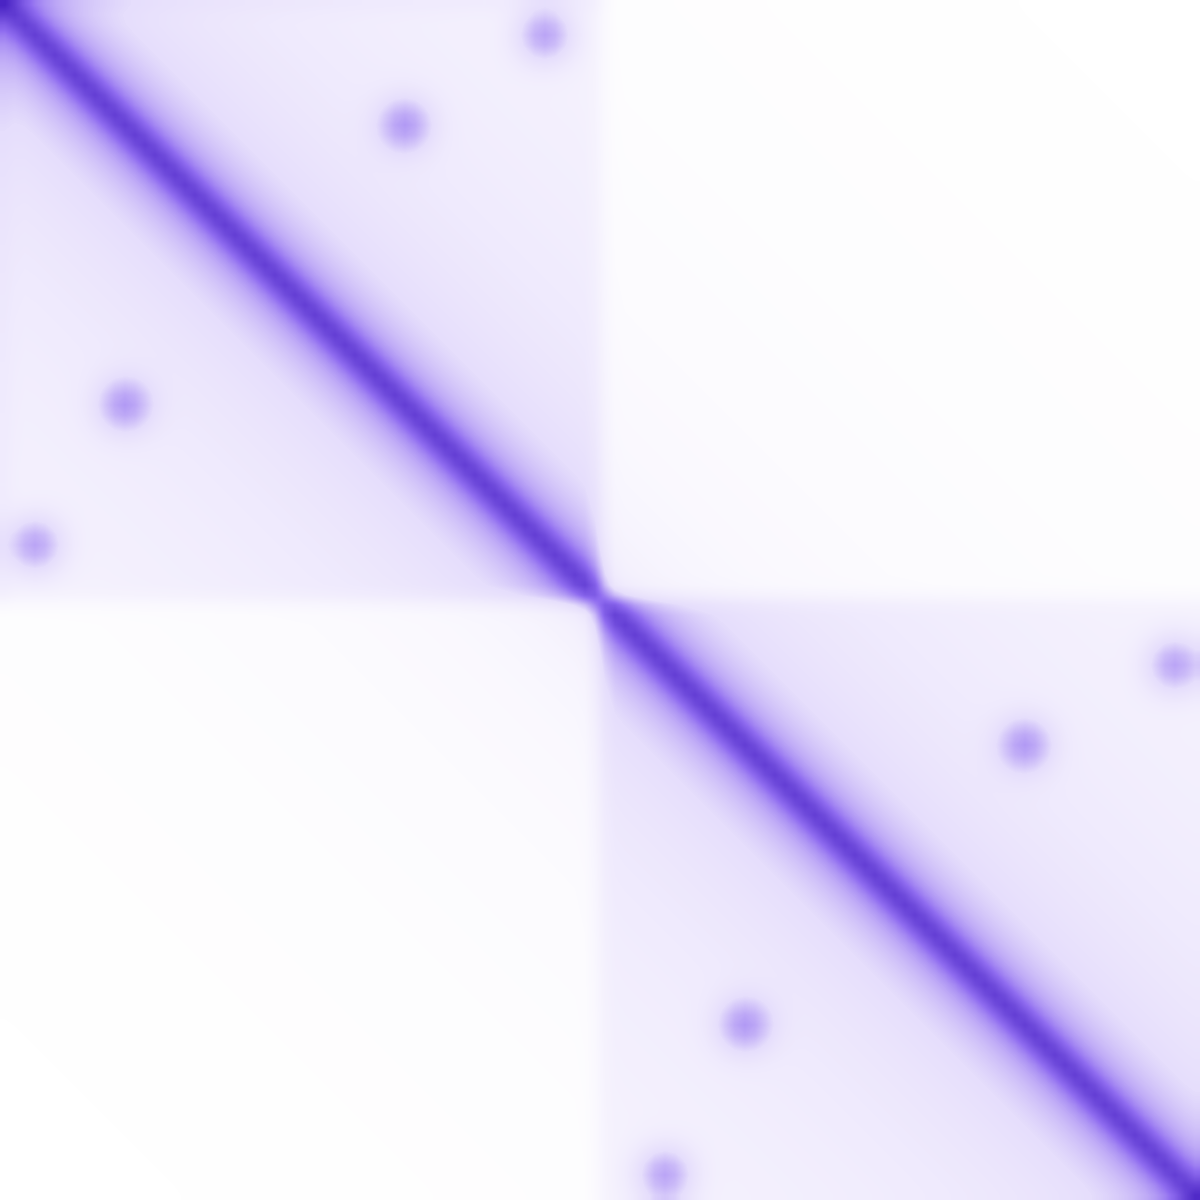
\includegraphics[width=\W cm]{tad_map.png}};
  \draw[ink!50,line width=0.7pt] (0,-1.2) rectangle (\W,{-1.2-\W});
  \draw[dashed,ink!45,line width=0.7pt] ({60*\u},0) --({60*\u},{-1.2-\W});
  % fibre with loops and CTCF
  \draw[fiber] (0,0)--(\W,0);
  \archx{3}{54}{lp}\archx{12}{40}{lp2}\archx{66}{117}{lp}\archx{74}{102}{lp2}
  \foreach \b/\o in {3/f,54/r,66/f,117/r}{\pgfmathsetmacro{\xx}{\b*\u}\prot{\xx}{0}{\o}}
  \node[note,anchor=east] at (-0.2,0) {fibre};
  \node[note,anchor=east] at (-0.2,-1.2) {contact map};
  % TAD tags on the map
  \node[font=\bfseries\small,text=ink] at ({24*\u},{-1.2-52*\u}) {TAD 1};
  \node[font=\bfseries\small,text=ink] at ({86*\u},{-1.2-113*\u}) {TAD 2};
  % call-outs on the right
  \pgfmathsetmacro{\xr}{\W+0.5}
  \node[lab,anchor=west,align=left] at (\xr,{-1.2-0.12*\W}) {\textbf{loop dot}\\[-1pt]{\footnotesize a stable loop holds its two}\\{\footnotesize anchors close together}};
  \draw[leader] (\xr-0.05,{-1.2-0.12*\W})--({40*\u+0.1},{-1.2-12*\u}) node[fill=ink,circle,inner sep=1.2pt] {};
  \node[lab,anchor=west,align=left] at (\xr,{-1.2-0.5*\W}) {\textbf{TAD boundary}\\[-1pt]{\footnotesize two CTCF sites facing apart:}\\{\footnotesize contacts stop here}};
  \draw[leader] (\xr-0.05,{-1.2-0.5*\W})--({60*\u},{-1.2-0.5*\W}) node[fill=ink,circle,inner sep=1.2pt] {};
  \node[lab,anchor=west,align=left] at (\xr,{-1.2-0.86*\W}) {\textbf{darker = more contacts}\\[-1pt]{\footnotesize nearby loci touch most often}};
\end{tikzpicture}
\end{document}
